\part{Basic texture mapping}
\frame{\partpage}

\begin{frame}{Shaders vs. textures}
	\begin{itemize}
		\pause\item \textbf{Shaders} determine surface appearance based on \textbf{interpolated per-vertex} properties.
		\pause\item \textbf{Textures} are 2D images (or arrays of values) that allow properties to be \textbf{varied across the surface}.
		\pause\item Values may represent colours, transparency, surface normals, surface displacements, light reflectance parameters etc.
		\pause\item \textbf{But} we can still only pass values at vertices...
	\end{itemize}
\end{frame}

\begin{frame}{Texture coordinates}
	\begin{itemize}
		\item We use \textbf{UV coordinates} to refer to points in a texture
		\pause\item $u$ axis is horizontal and ranges from 0 (left) to 1 (right)
		\pause\item $v$ axis is vertical and ranges from 0 (bottom) to 1 (top)
		\pause\item (So really just another name for $xy$ coordinates in texture space)
		\pause\item Basic idea of texture mapping: give each vertex a $uv$ coordinate, and interpolate across the triangle
	\end{itemize}
\end{frame}

\begin{frame}{UV coordinates}
	\begin{center}
		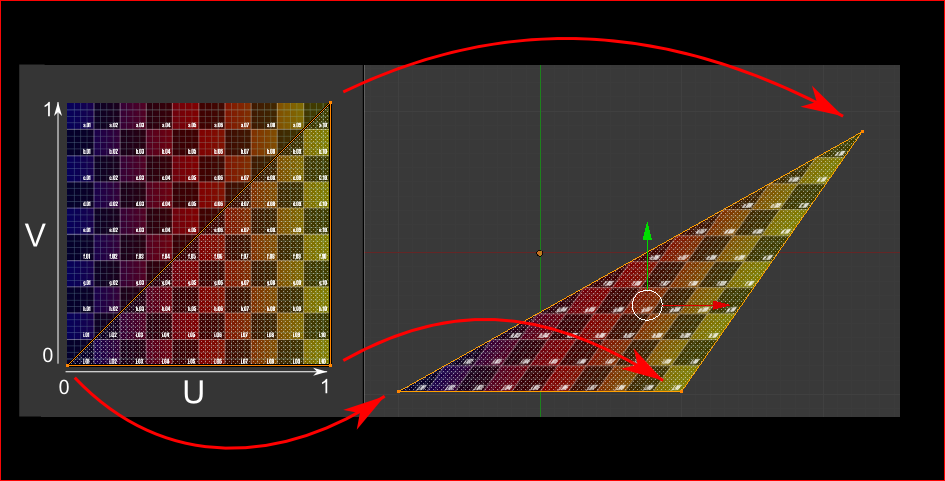
\includegraphics[width=\textwidth]{uv}
	\end{center}
\end{frame}

\begin{frame}{Character textures}
	\begin{center}
		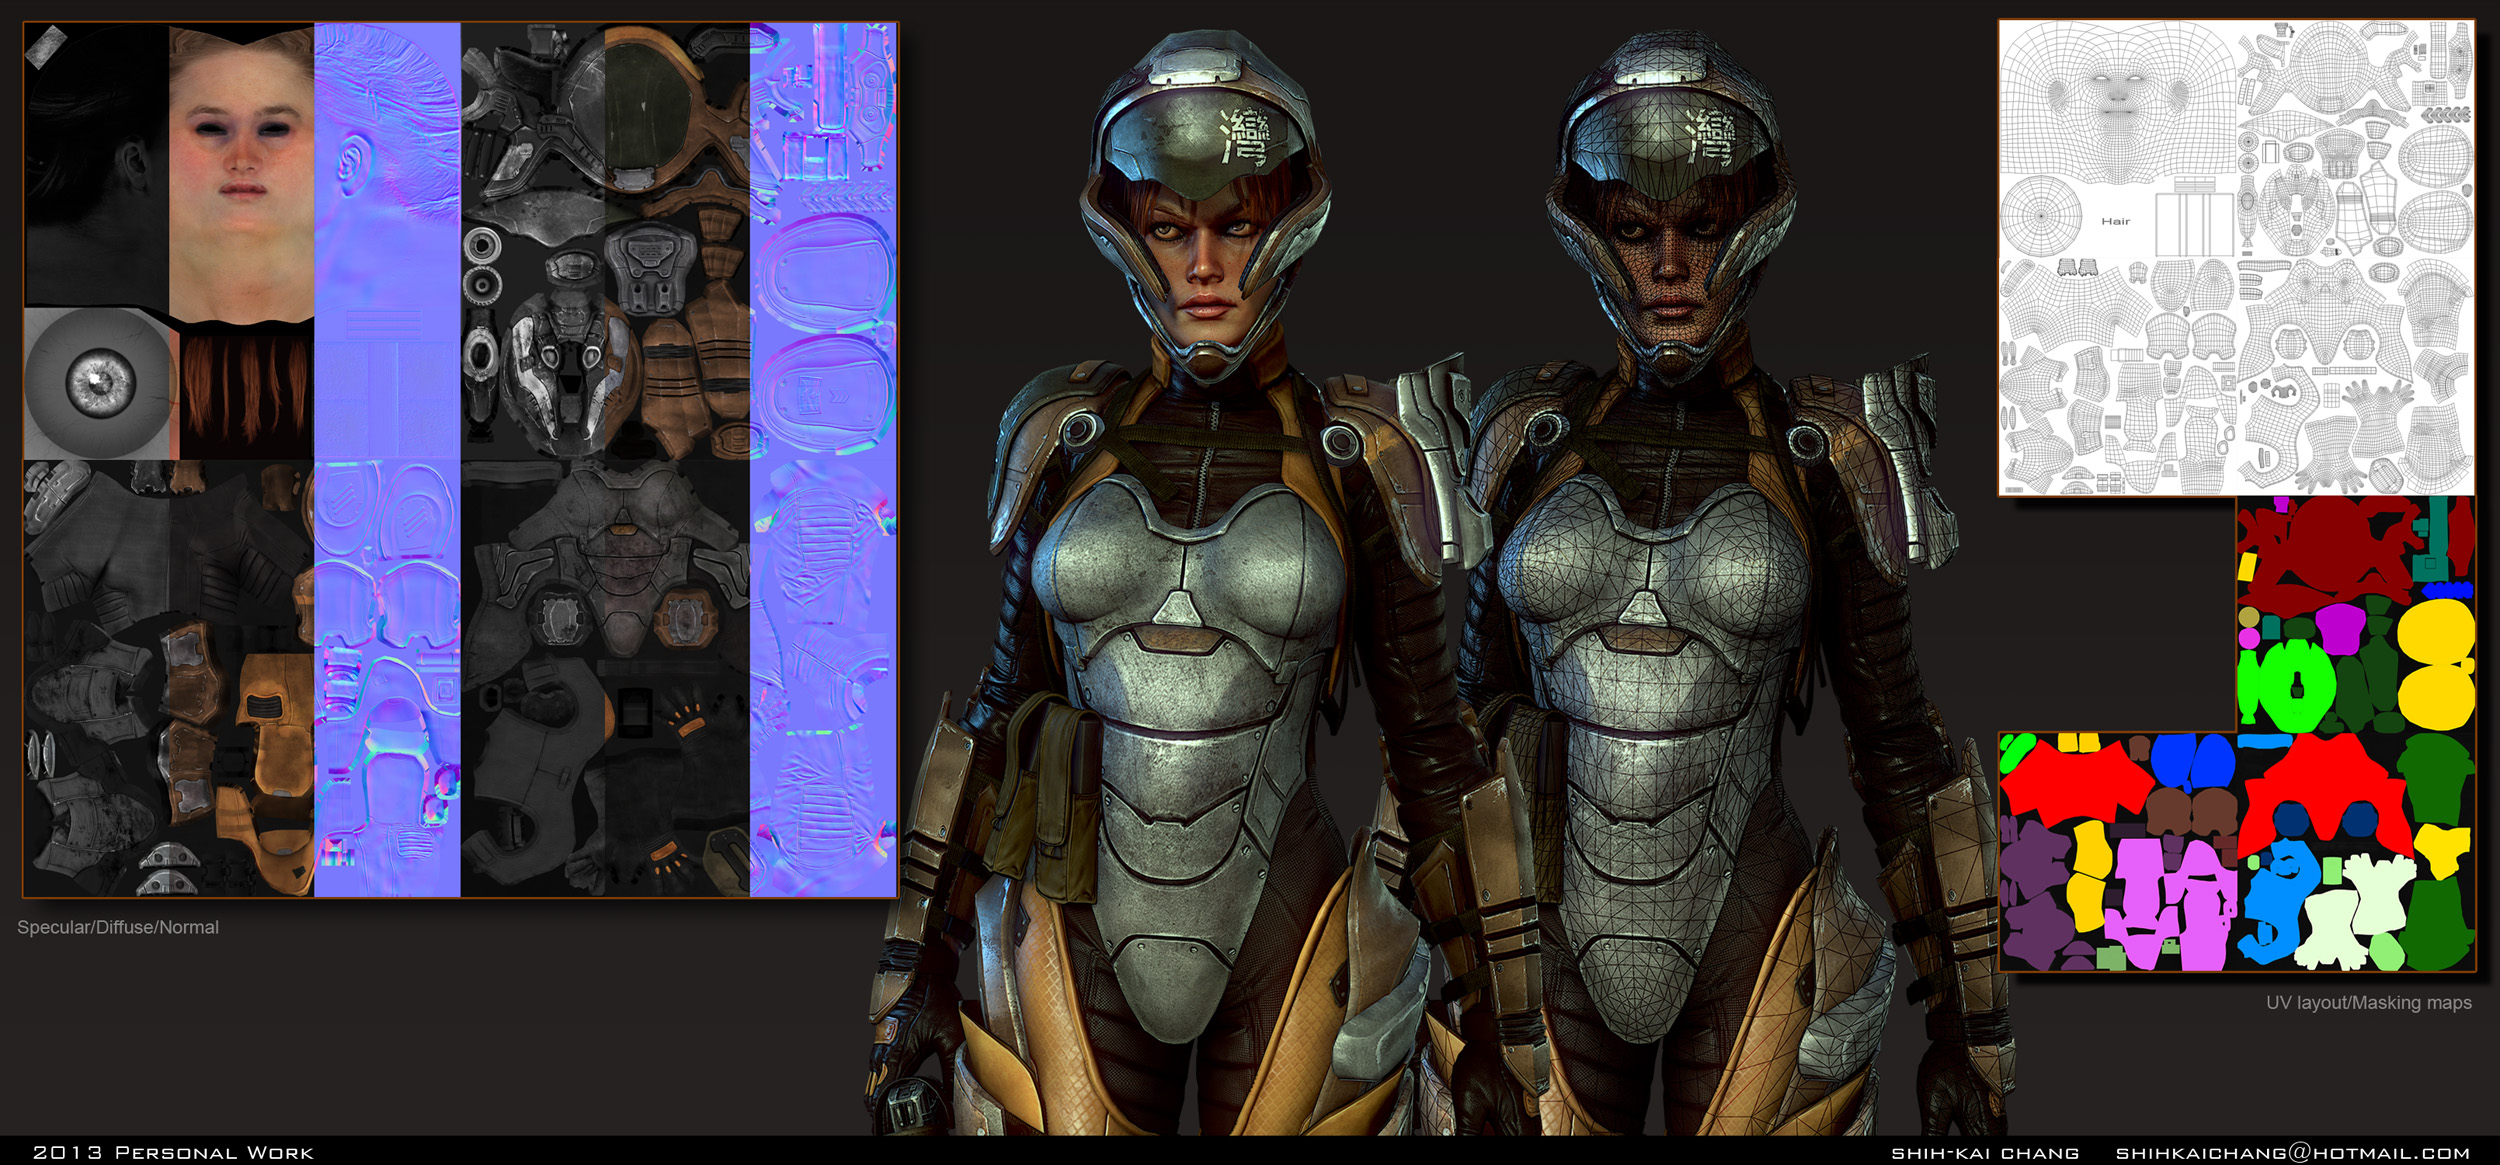
\includegraphics[width=\textwidth]{character_texture}
	\end{center}
\end{frame}

\part{Texture parameters}
\frame{\partpage}

\begin{frame}{Texture wrapping}
	What happens if we assign a coordinate outside the $uv$ range?
	\begin{itemize}
		\pause\item The \textbf{wrapping} parameter determines what happens for texture coordinates < 0 or > 1
	\end{itemize}
	\begin{figure}[h!]
		\pause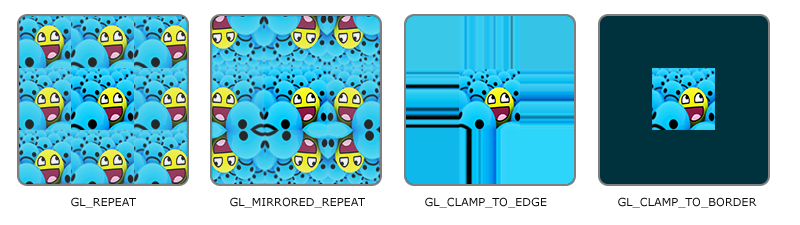
\includegraphics[width=\textwidth]{texture_wrapping}
		\caption*{Image source: \url{https://learnopengl.com/Getting-started/Textures}}
	\end{figure}
\end{frame}

\begin{frame}{Texture filtering}
	How do we map a floating-point texture coordinate to the correct \textbf{texel} (texture element)?
	\begin{itemize}
		\pause\item \textbf{Nearest neighbour} selects the texel with the closest centre (Manhattan distance).
		\pause\item \textbf{(Bi)linear} takes an interpolated value from neighbouring texels.
		\pause\item Can specify different modes for scaling up and down.
	\end{itemize}
	\begin{center}
		\begin{figure}[h!]
			\pause
\includegraphics[width=0.3\textwidth]{texture_filtering}
			\caption*{Image source: \url{https://learnopengl.com/Getting-started/Textures}}
		\end{figure}
	\end{center}
\end{frame}

\begin{frame}{Mipmaps}
	On faraway objects, a fragment may cover many texels...
	\begin{itemize}	
		\pause\item A \textbf{mipmap} is a set of textures with each scaled to half the size of the last.
		\pause\item Chosen based on the distance to the camera.
		\pause\item "Multum in parvo" = "much in a small space"
		\pause\item Pregenerated (on request) by OpenGL: faster processing/better quality for more memory.
	\end{itemize}
	\begin{center}
		\begin{figure}[h!]
			\pause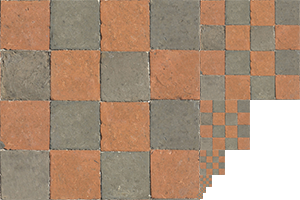
\includegraphics[width=0.3\textwidth]{mipmaps}
			\caption*{Image source: \url{https://learnopengl.com/Getting-started/Textures}}
		\end{figure}
	\end{center}
\end{frame}

\begin{frame}{Texture dimensions}
	\begin{itemize}
		\item In the old days, OpenGL required textures to have \textbf{power of two} dimensions
			\begin{itemize}
				\pause\item $2, 4, 8, 16, 32, 64, 128, 256, 512, 1024, \dots$
			\end{itemize}
		\pause\item Nowadays \textbf{non-power of two (NPOT)} textures are widely supported
		\pause\item Still better to stick to powers of two as some things work better (e.g.\ mipmapping)
		\pause\item NB: \textbf{rectangular} textures are fine, but \textbf{square} textures make UV coordinates saner
	\end{itemize}
\end{frame}